\documentclass[journal]{IEEEtran}
\usepackage{amsmath,amsfonts}
\usepackage{algorithmic}
\usepackage{algorithm}
\usepackage{array}
\usepackage{textcomp}
\usepackage{stfloats}
\usepackage{url}
\usepackage{verbatim}
\usepackage{graphicx}
\usepackage{cite}
\hyphenation{op-tical net-works semi-conduc-tor IEEE-Xplore}
% updated with editorial comments 8/9/2021

% custom
\usepackage{color}
\usepackage{booktabs}
\usepackage{threeparttable}
\usepackage{multirow}
\usepackage{makecell}
\usepackage{float}
\usepackage{siunitx}

\newcommand{\degree}{^\circ}
\newcommand{\etal}{\textit{et al.}}
\newcommand{\hhline}{\noalign{\vskip 1pt}\hline\noalign{\vskip 1pt}}

\makeatletter
\let\MYcaption\@makecaption
\makeatother
\usepackage[font=scriptsize]{subcaption}
\makeatletter
\let\@makecaption\MYcaption
\makeatother

\begin{document}
	
\title{How to Use \LaTeX\ Draw Beautiful Charts}

\author{XXX, 
	XXX, ~\IEEEmembership{Member, IEEE}, 
	and XXX, ~\IEEEmembership{Senior Member, IEEE}
	
	\IEEEcompsocitemizethanks{\IEEEcompsocthanksitem
		This work was supported in part by the XXX under Grant 123456.
		The authors are with XXX (e-mail: XXX; XXX; XXX).
	}
}

% The paper headers
\markboth{Journal of \LaTeX\ Class Files,~Vol.~14, No.~8, August~2021}%
{XXX \MakeLowercase{\textit{et al.}}: XXX}

% \IEEEpubid{0000--0000/00\$00.00~\copyright~2021 IEEE}
% Remember, if you use this you must call \IEEEpubidadjcol in the second
% column for its text to clear the IEEEpubid mark.

\maketitle


\section{Example}
\begin{table*}[!ht] 
	\caption{All fingerprint datasets used in experiments.}
	\label{tab:datasets}
	\vspace{-0.7cm}
	\begin{center}
		\begin{threeparttable}
			\begin{tabular}{p{.12\linewidth}<{\centering}*{1}{p{.24\linewidth}<{\centering}}*{1}{p{.14\linewidth}<{\centering}}*{1}{p{.24\linewidth}<{\centering}}*{1}{p{.14\linewidth}<{\centering}}}
				\toprule
				\multirow{2}{*}{Database} 	
				& \multicolumn{2}{c}{Hisign Latent}
				& TDF
				& THU Old \\
				\cmidrule(lr){2-3} \cmidrule(lr){4-4} \cmidrule(lr){5-5}
				& Rolled / Plain
				& Latent
				& Plain
				& Plain \\
				\midrule
				Image                     & \raisebox{-.5\height}{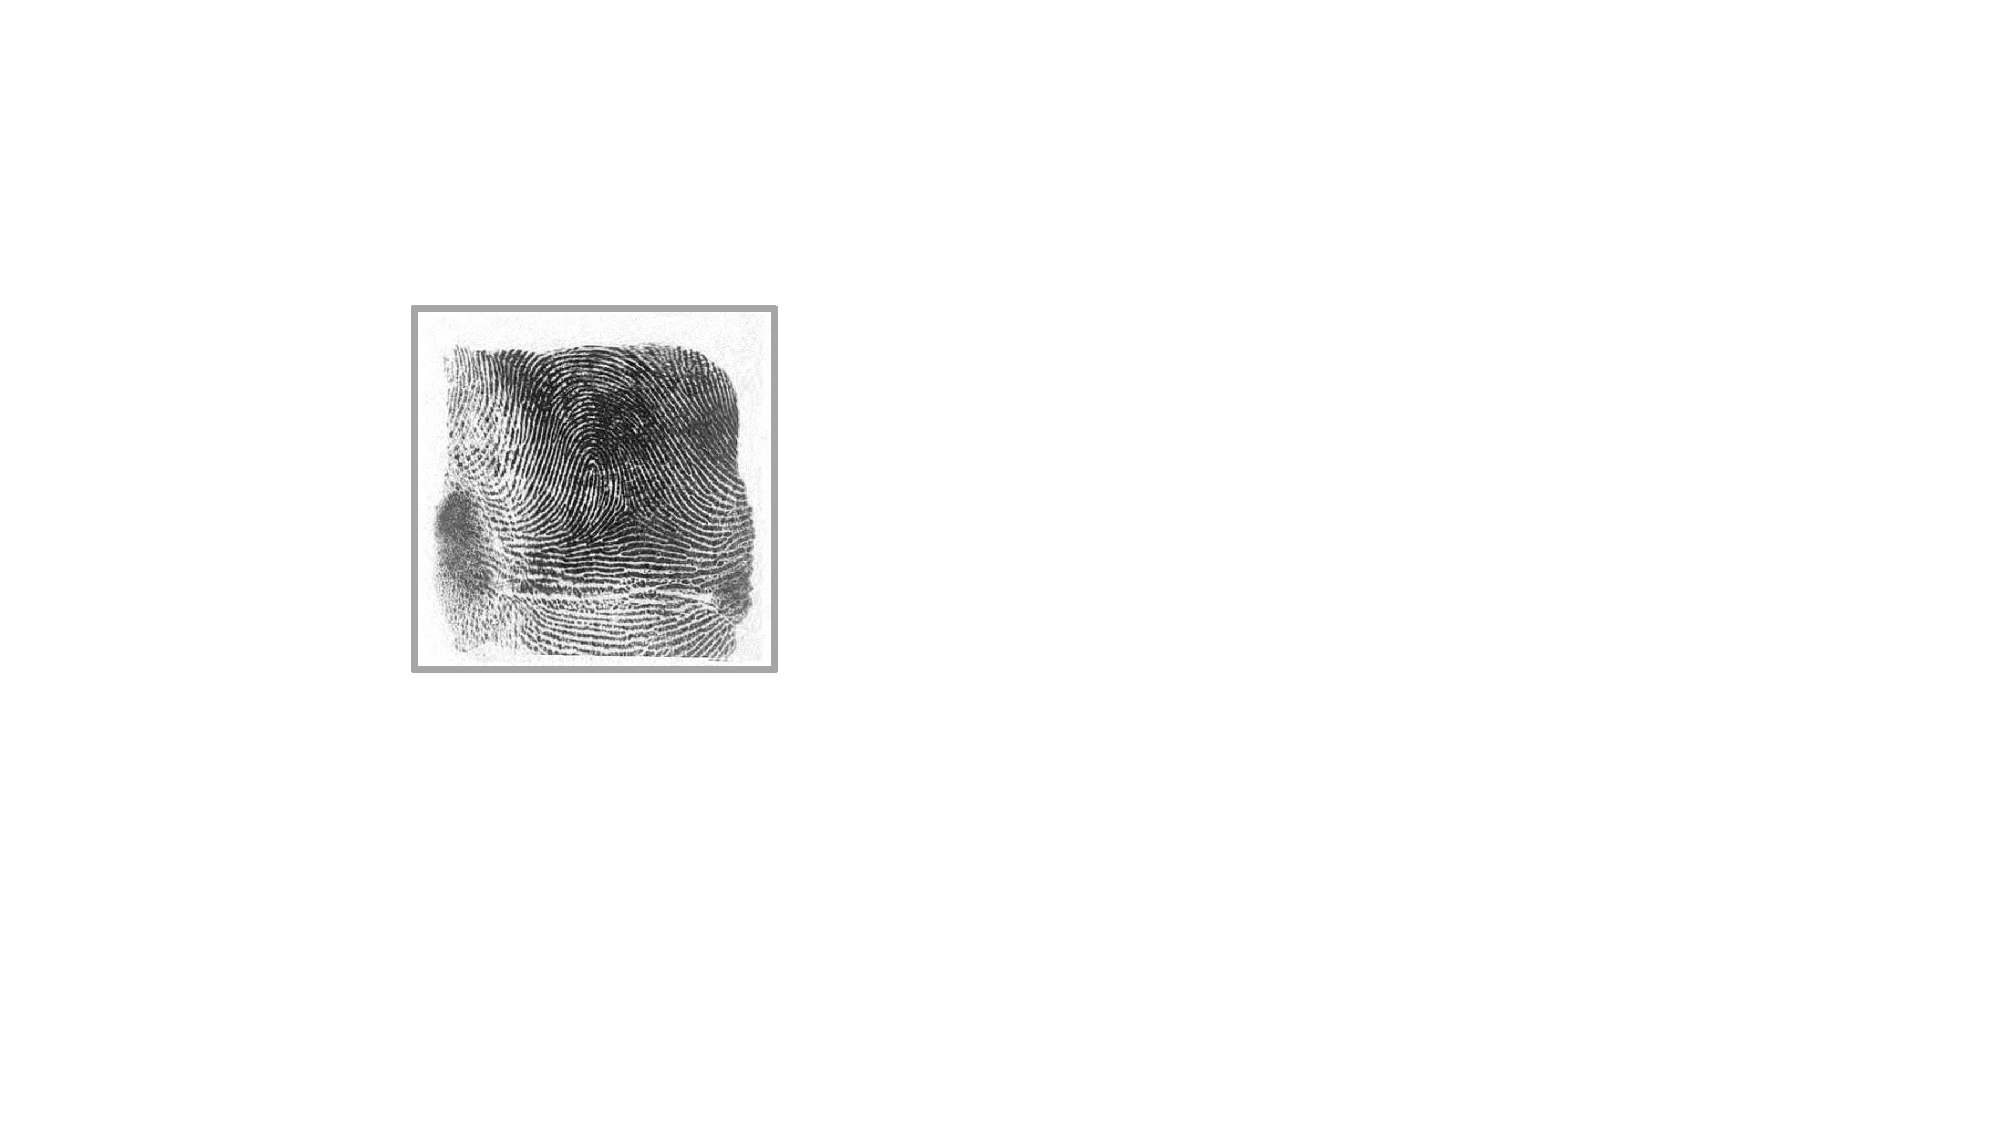
\includegraphics[height=.8in]{images/datasets/Hisign_latent_file2.pdf}}~\raisebox{-.5\height}{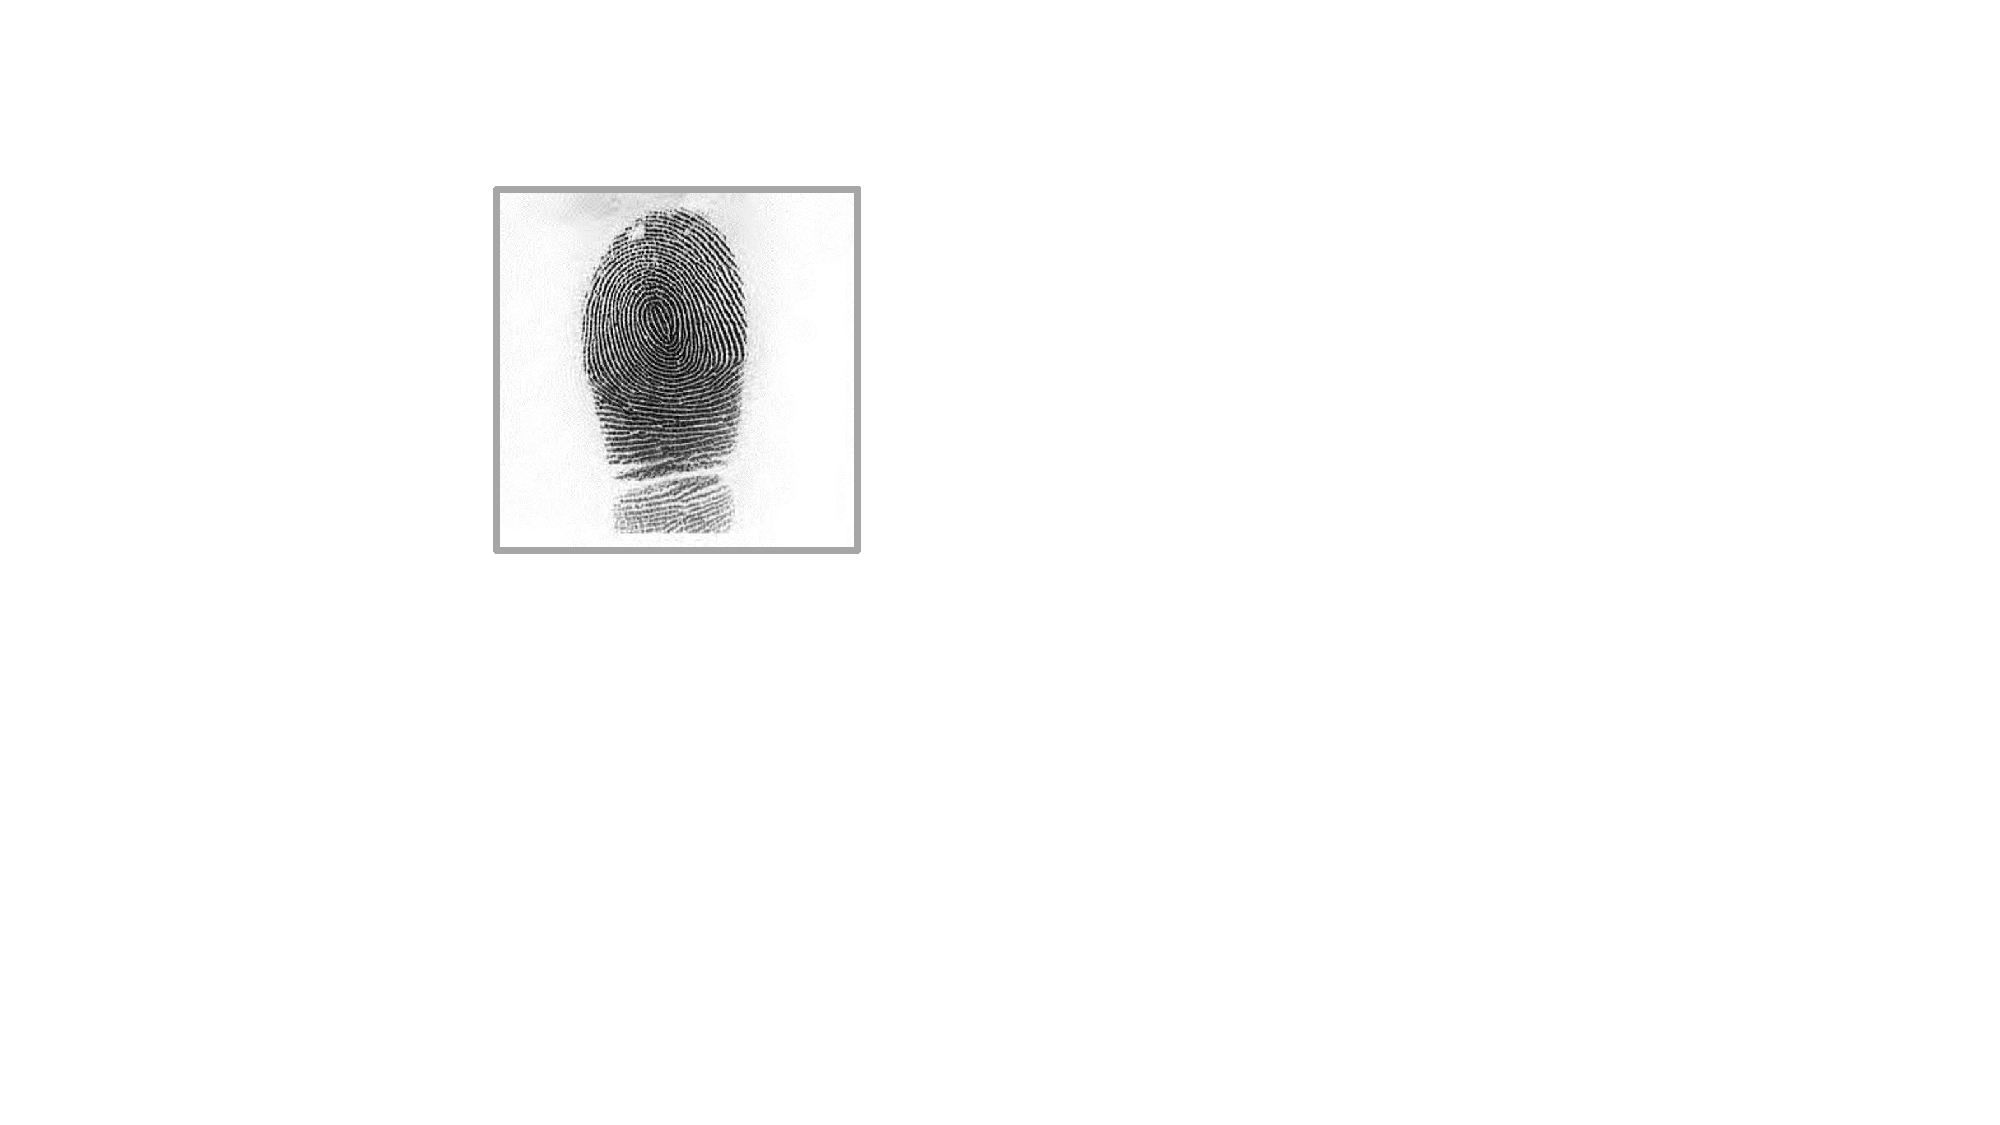
\includegraphics[height=.8in]{images/datasets/Hisign_latent_file1.pdf}}
				& \raisebox{-.5\height}{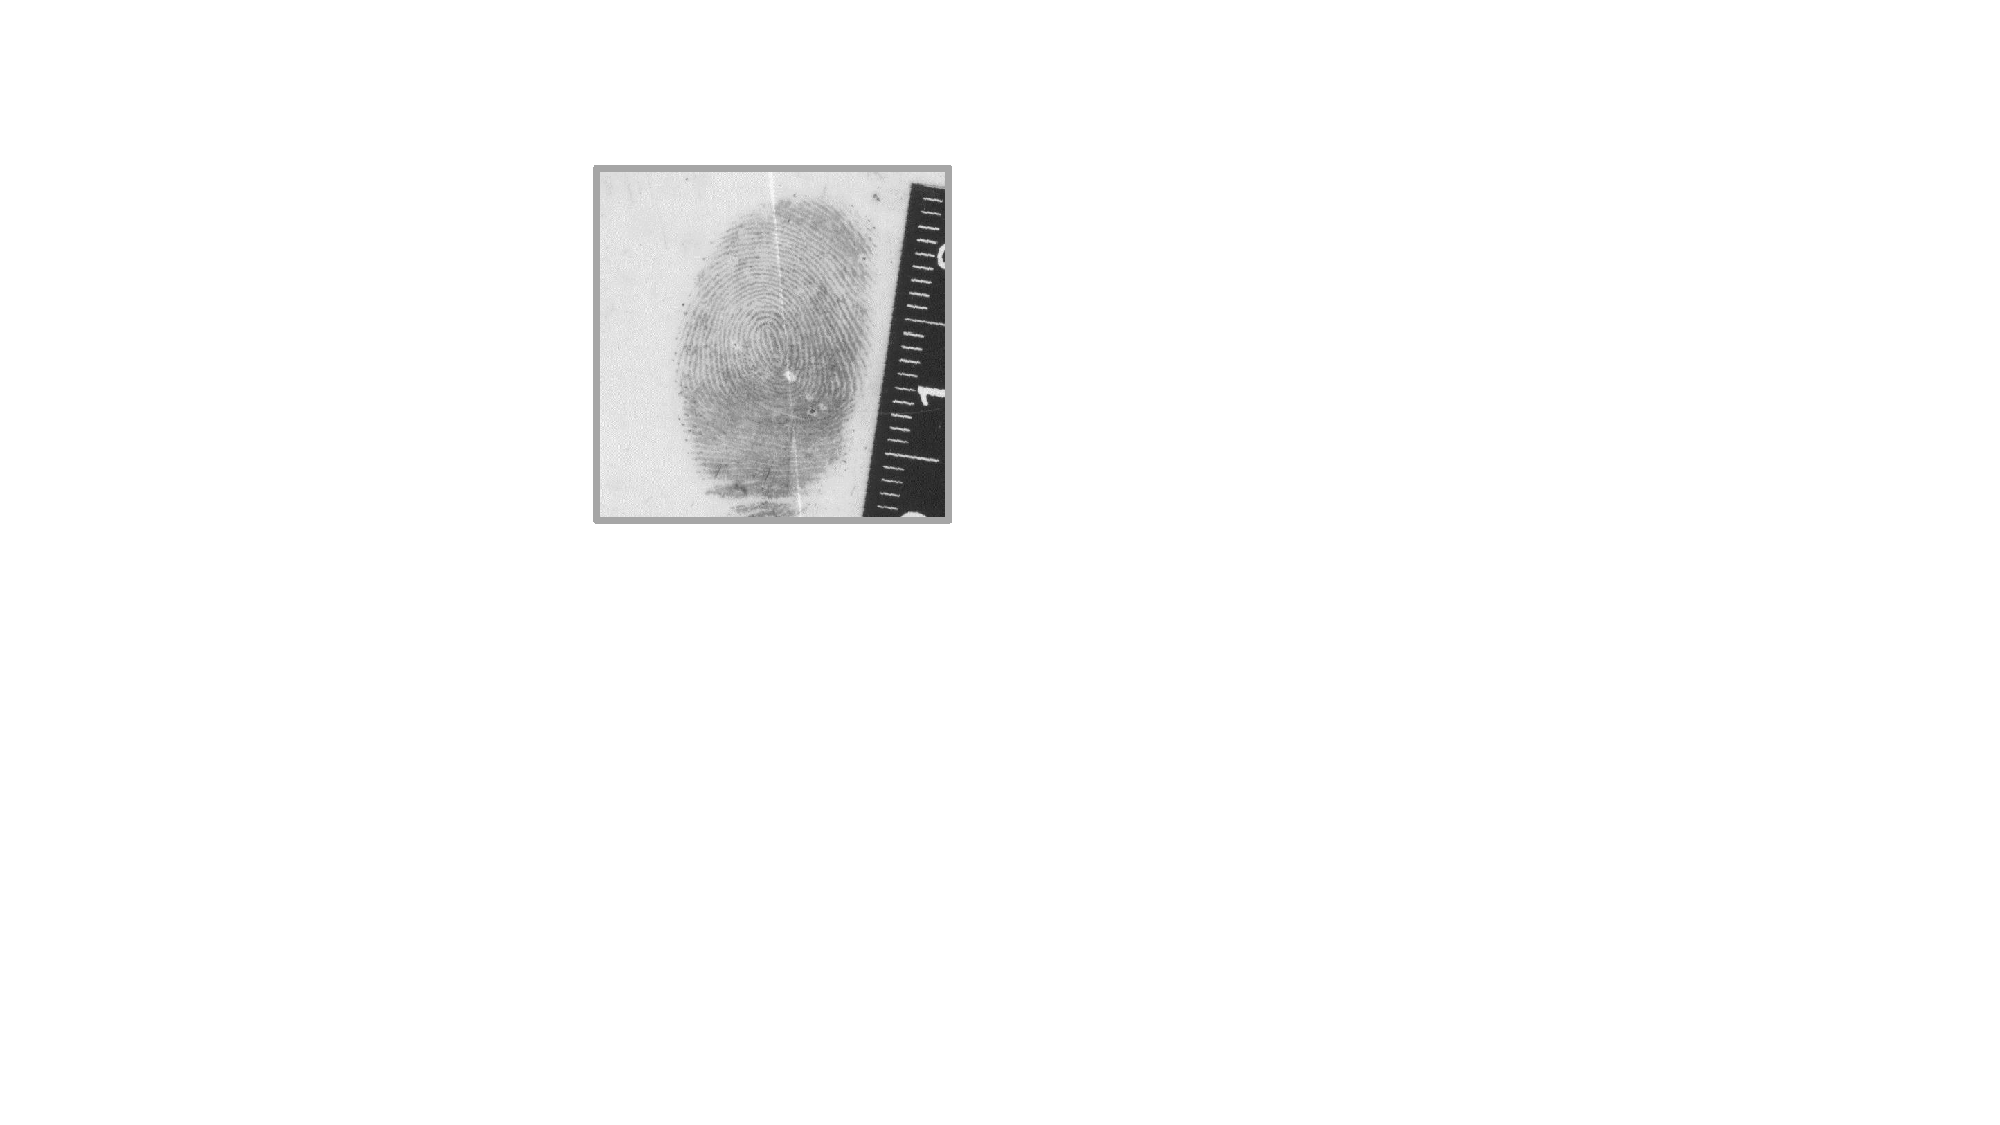
\includegraphics[height=.8in]{images/datasets/Hisign_latent_latent.pdf}}
				& \raisebox{-.5\height}{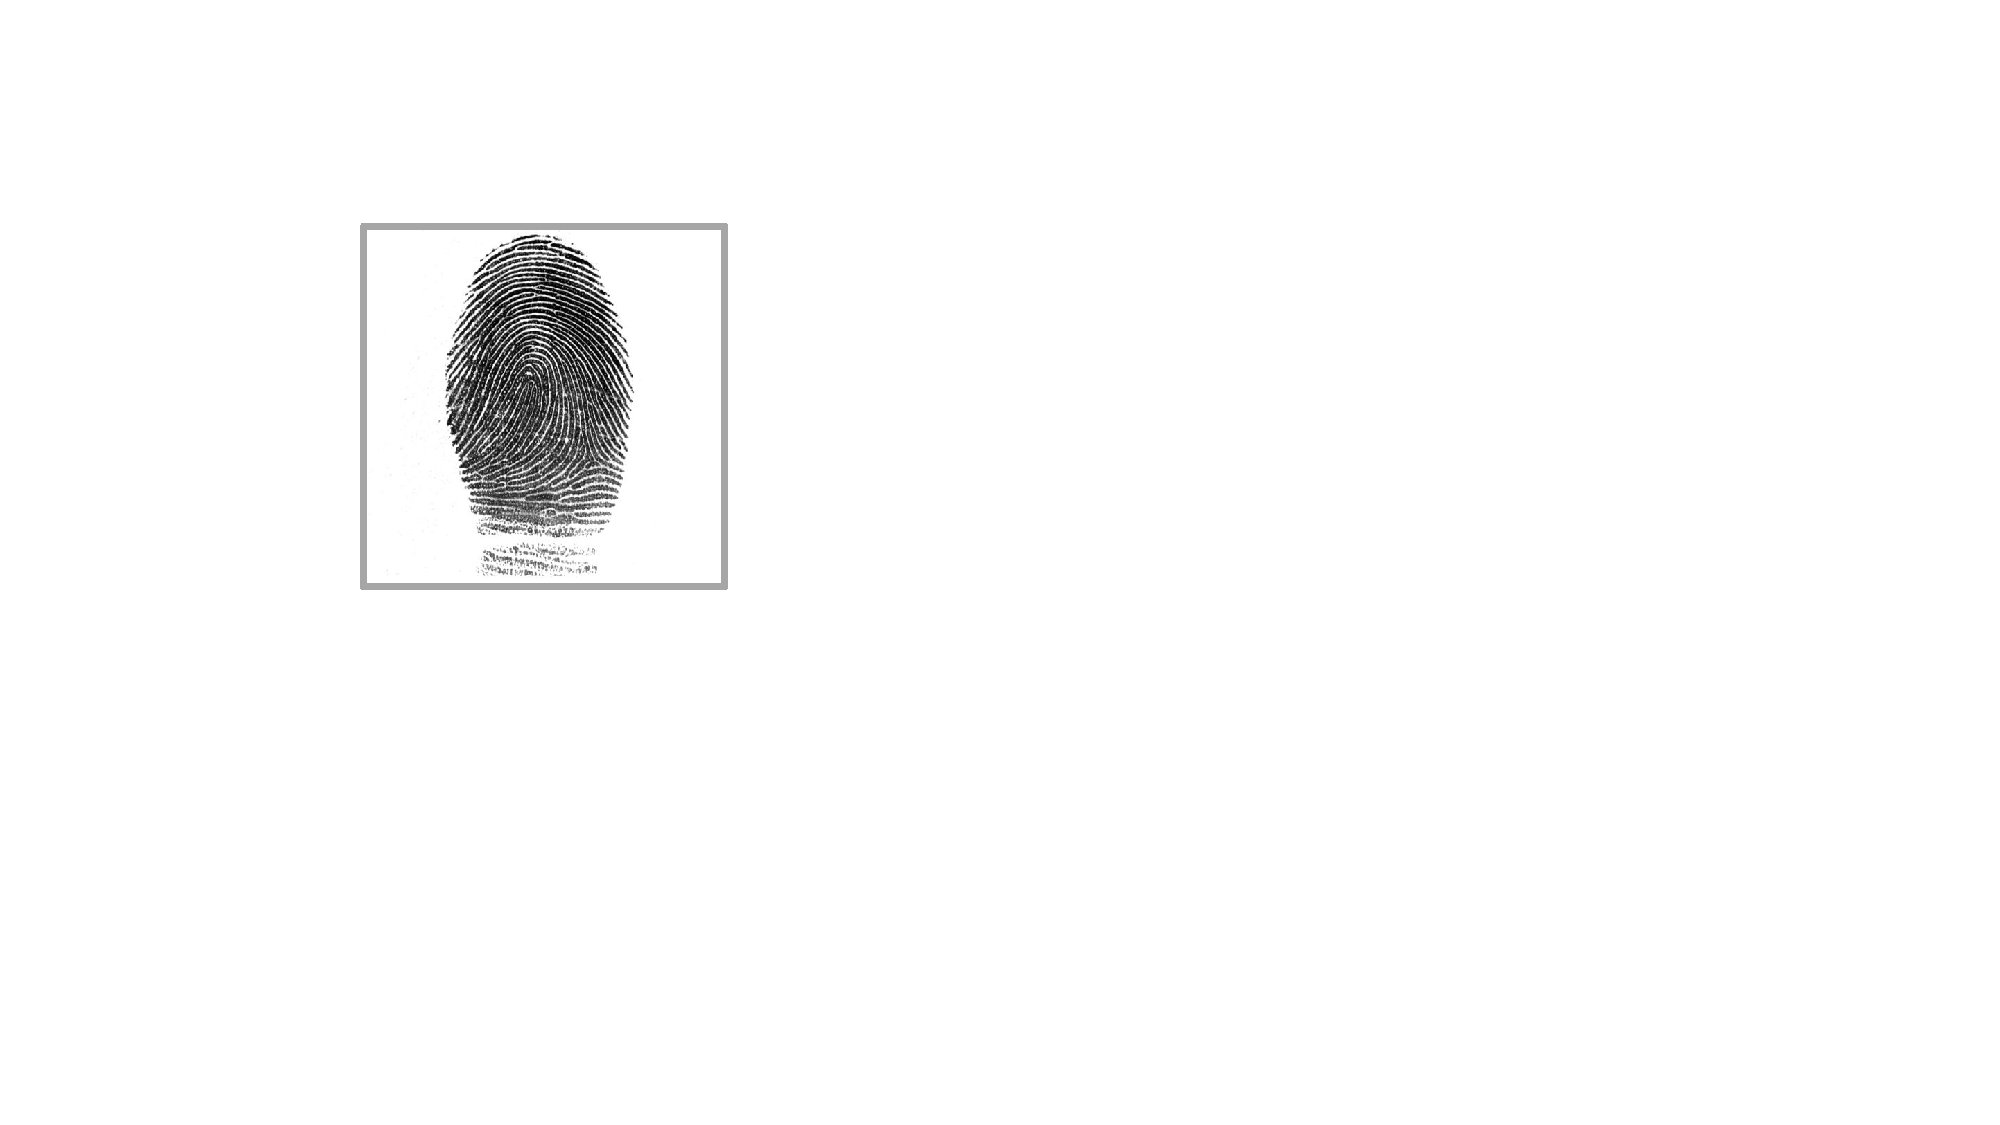
\includegraphics[height=.8in]{images/datasets/TDF_0.pdf}}~\raisebox{-.5\height}{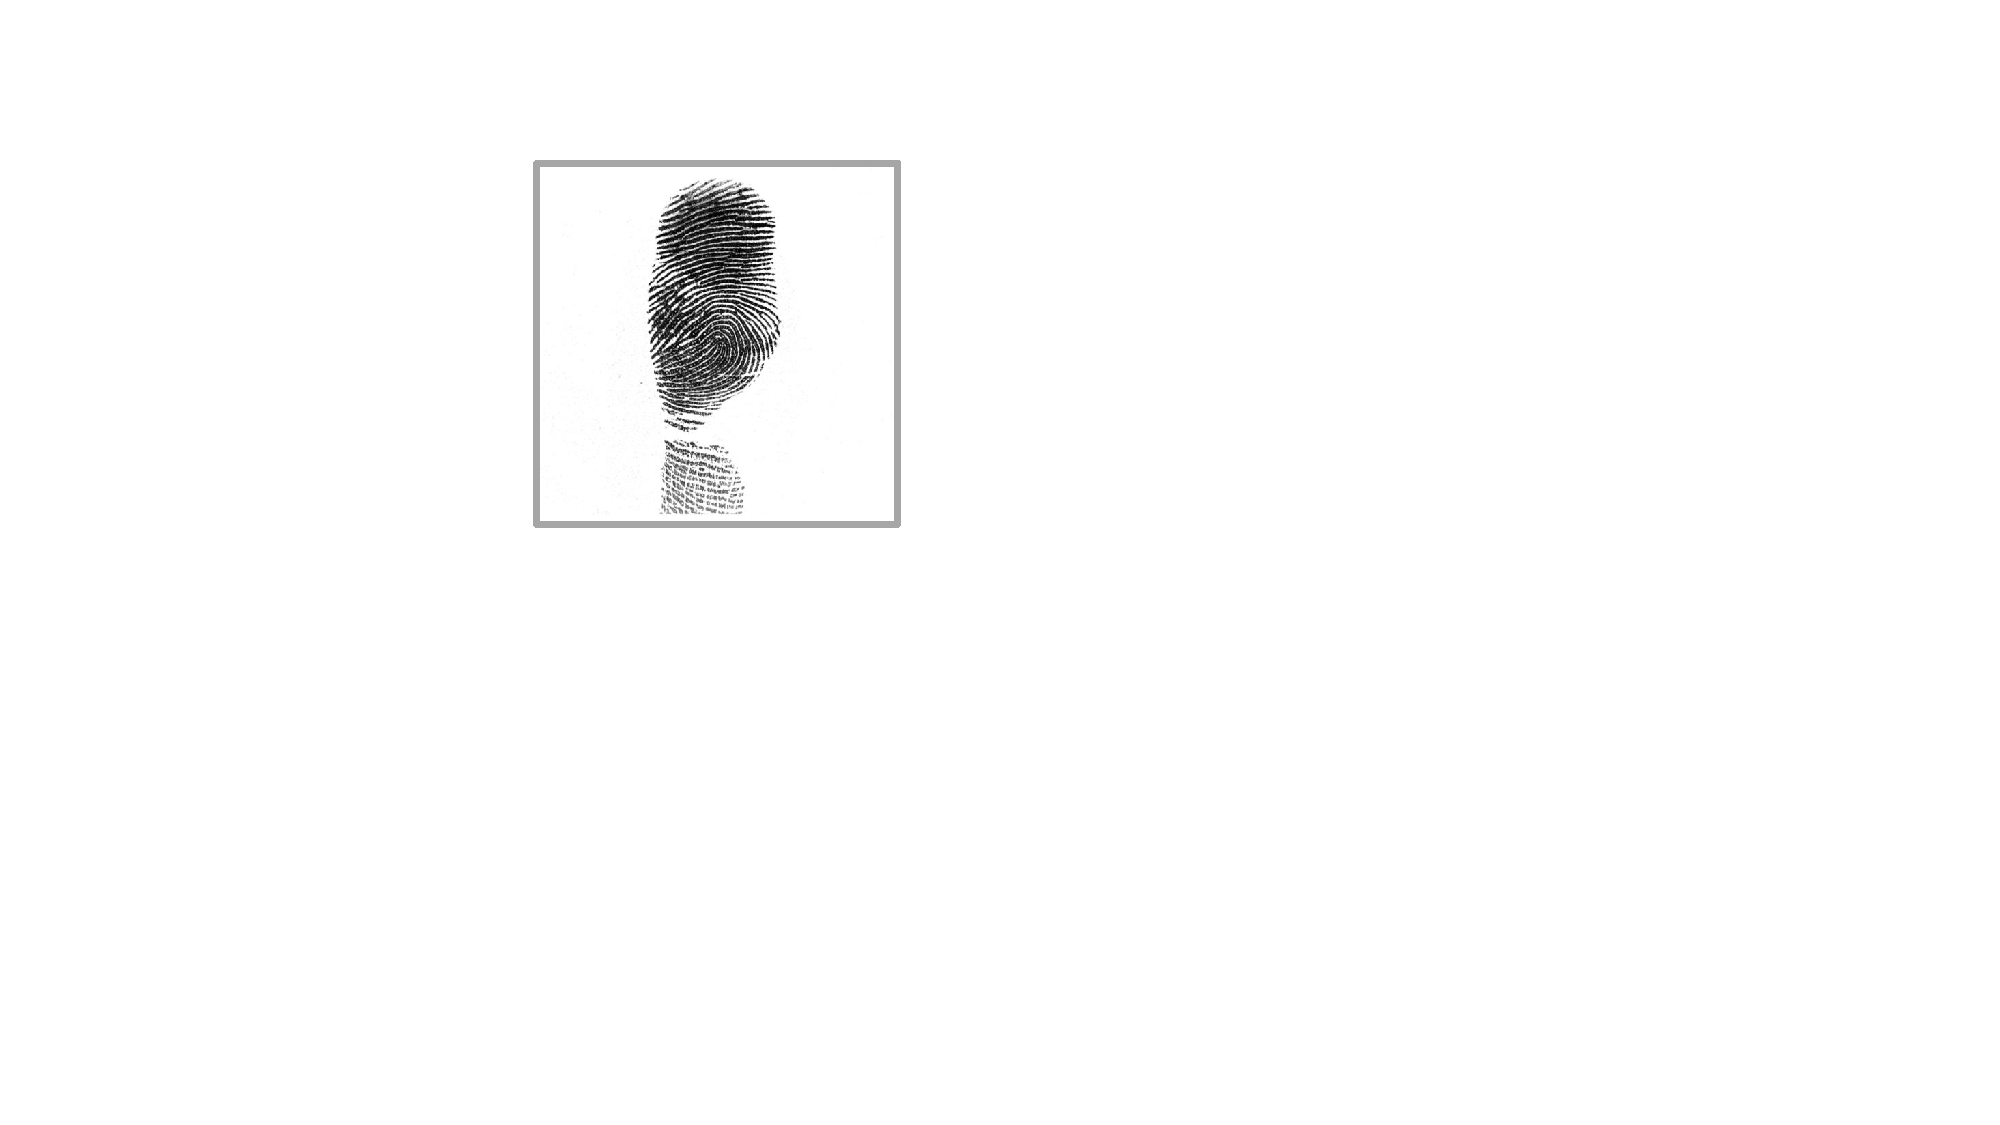
\includegraphics[height=.8in]{images/datasets/TDF_1.pdf}}
				& \raisebox{-.5\height}{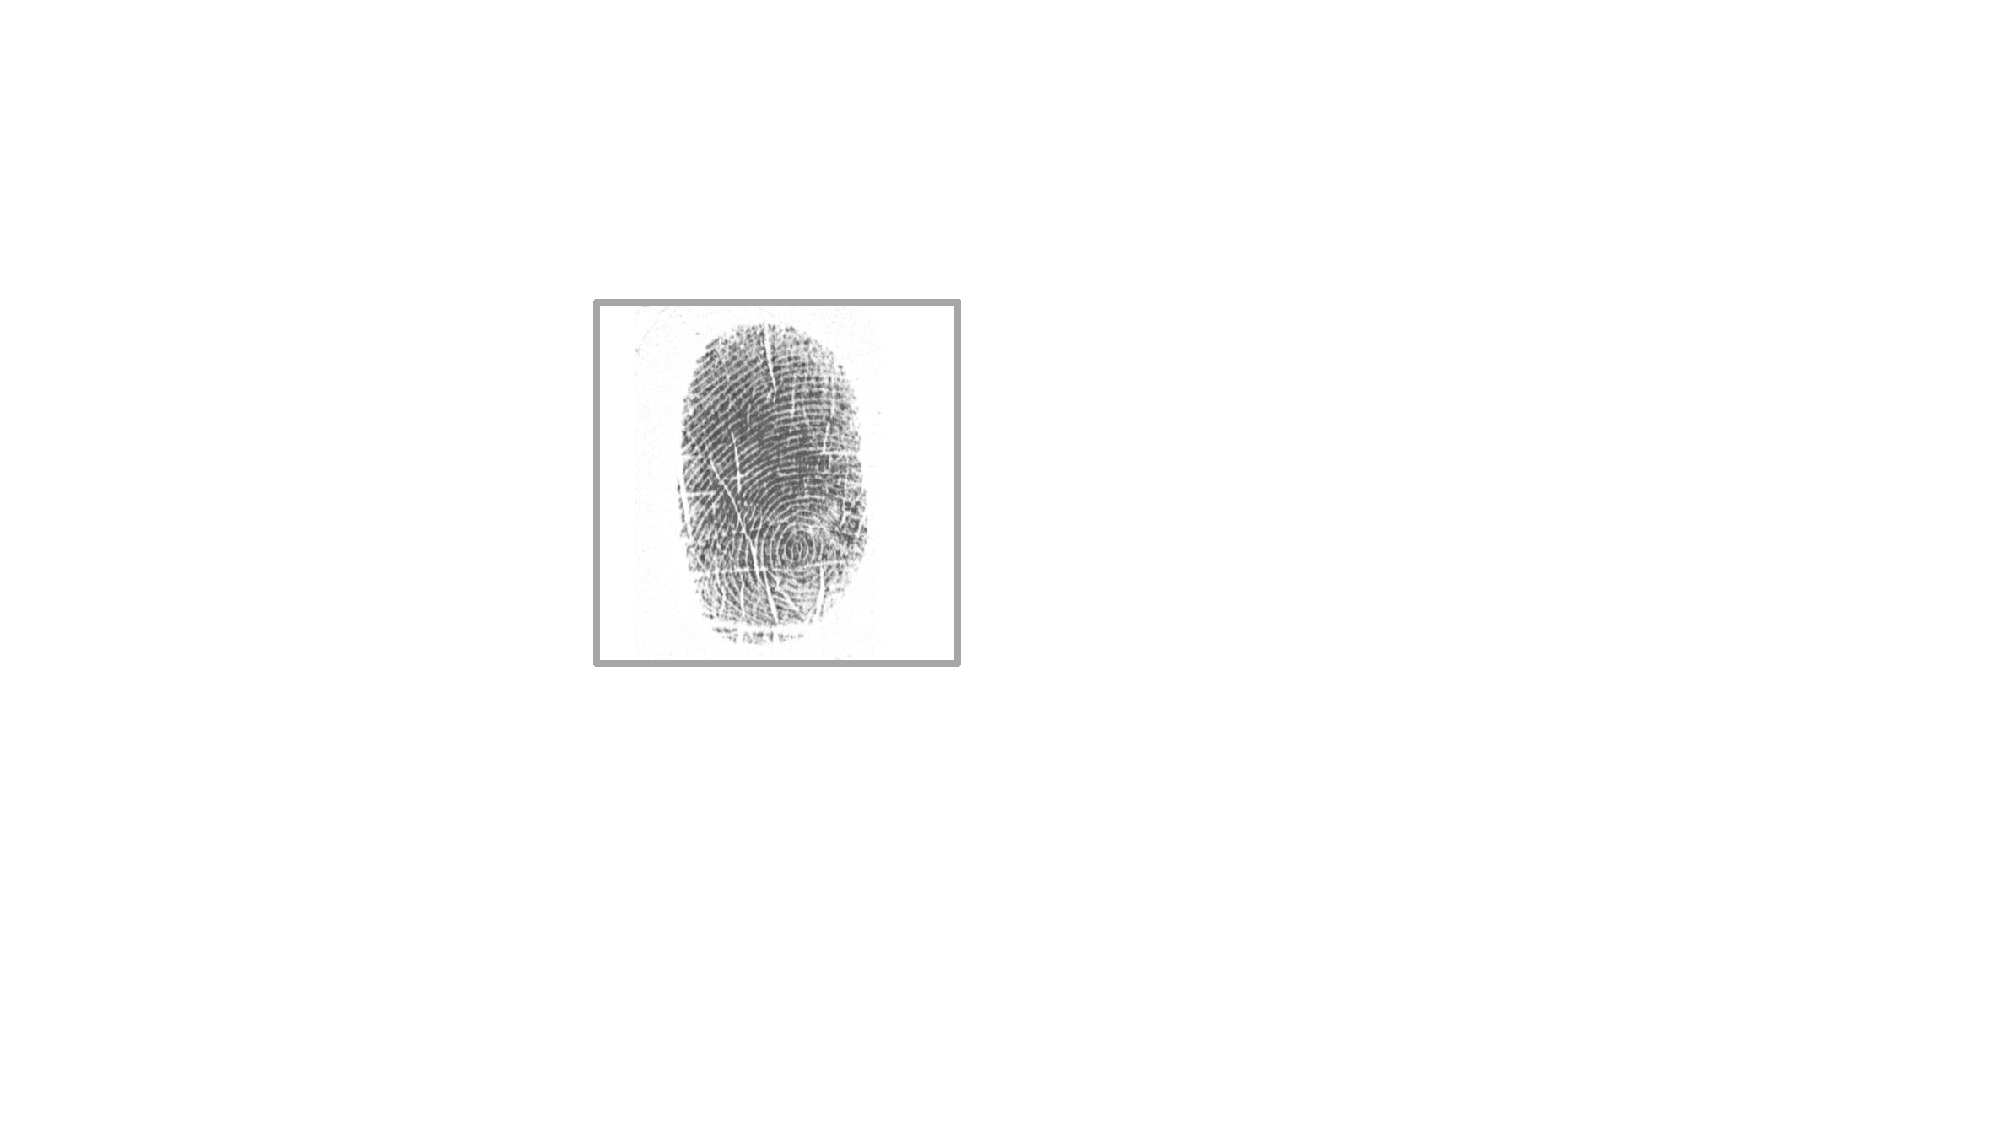
\includegraphics[height=.8in]{images/datasets/THU_OLD.pdf}} \\
				\hhline
				Sensor
				& Inking / Optical                    
				& -
				& Optical
				& Optical \\
				\hhline
				Description              
				& \multicolumn{2}{c}{\makecell{10459 pairs \\ latent fingerprints from real crime scenes}}
				& \multicolumn{1}{c}{\makecell{320 videos \\ large distortion}}
				& \multicolumn{1}{c}{\makecell{136 fingers $\times$ 2\\ wrinkled and low quality}}\\
				\hhline
				Usage                     
				& \multicolumn{2}{c}{Training}
				& Training
				& \multicolumn{1}{c}{\makecell{Registration accuracy\\Matching performance}} \\
				\hhline
				Genuine Match
				& \multicolumn{2}{c}{$\backslash$}
				& $\backslash$
				& 136\tnote{a}\\
				\hhline
				Imposter Match
				& \multicolumn{2}{c}{$\backslash$}
				& $\backslash$ 
				& 9,180\tnote{b}\\
				\bottomrule
			\end{tabular}
			\vspace*{0.25mm}
			
			
			\begin{tablenotes}
				\item[a] Each fingerprint is matched with other fingerprints from the same finger. The symmetric matches are avoided.
				\item[b] First fingerprints of each finger are matched each other. The symmetric matches are avoided.
				\item[c] Each latent fingerprint is matched with all rolled fingerprints from other fingers.
				
			\end{tablenotes}
		\end{threeparttable}
	\end{center}
\end{table*}

\begin{table*}[!t]
	\caption{Matching Performance by Image Correlator with Different Fingerprint Registration Algorithms}
	\label{tab:matching_corr}
	\vspace{-0.4cm}
	\begin{center}
		\begin{threeparttable}
			\begin{tabular}{p{.14\linewidth}<{\raggedright}*{18}{p{.022\linewidth}<{\centering}}}
				\toprule
				\multirow{2}*[-3pt]{\textbf{Method}}            
				& \multicolumn{3}{c}{\scriptsize\textbf{FVC2004 DB1\_A}}         
				& \multicolumn{3}{c}{\scriptsize\textbf{FVC2004 DB1\_A*}}         
				& \multicolumn{3}{c}{\scriptsize\textbf{FVC2004 DB3\_A} }        
				& \multicolumn{3}{c}{\scriptsize\textbf{THU Old}}       
				& \multicolumn{3}{c}{\scriptsize\textbf{Hisign C2CL(CL-CL)}}                  
				& \multicolumn{3}{c}{\scriptsize\textbf{Hisign C2CL(C-CL)}} \\
				\cmidrule(lr){2-4}\cmidrule(lr){5-7}\cmidrule(lr){8-10}\cmidrule(lr){11-13}\cmidrule(lr){14-16}\cmidrule(lr){17-19}
				& \scriptsize{TAR} & \scriptsize{FMR} & \scriptsize{EER}
				& \scriptsize{TAR} & \scriptsize{FMR} & \scriptsize{EER}
				& \scriptsize{TAR} & \scriptsize{FMR} & \scriptsize{EER}
				& \scriptsize{TAR} & \scriptsize{FMR} & \scriptsize{EER}
				& \scriptsize{TAR} & \scriptsize{FMR} & \scriptsize{EER}
				& \scriptsize{TAR} & \scriptsize{FMR} & \scriptsize{EER} \\
				\midrule
				\multirow{1}{*}{TPS Based} 
				& 70.2 & 33.8 & 11.5
				& 72.6 & 46.9 & 11.6
				& 74.6 & 65.4 & 10.4
				& 70.6 & 37.2 & 11.7
				& 61.4 & 78.1 & 12.5
				& 45.3 & 99.6 & 22.3 \\
				\multirow{1}{*}{Phase Based}
				& 97.8 & 3.16 & 1.12
				& 98.7 & 2.78 & 0.64
				& 93.1 & 9.23 & 1.79
				& 94.9 & 9.53 & 3.68
				& 97.8 & \textbf{13.0} & 0.96
				& 96.2 & 48.3 & 1.17\\
				\multirow{1}{*}{DRN (local)\tnote{\dag}}
				& 91.1 & 25.5 & 2.49
				& 87.2 & 20.8 & 2.75
				& 72.5 & 46.4 & 5.98
				& 76.5 & 53.5 & 8.65
				& 71.8 & 82.7 & 5.75
				& 67.0 & 92.3 & 6.67\\
				\multirow{1}{*}{DRN (global)\tnote{\dag}}
				& 95.4 & 12.1 & 2.42
				& 97.5 & 8.00 & 1.10
				& 91.8 & 30.1 & 2.01
				& 91.9 & 14.7 & 2.21
				& 95.8 & 28.2 & 1.25
				& 95.3 & 42.8 & 1.19\\
				\midrule
				\multirow{1}{*}{Proposed\tnote{\dag}}
				& \textbf{98.9} & \textbf{1.54} & \textbf{0.79}
				& \textbf{99.8} & \textbf{0.41} & \textbf{0.17}
				& \textbf{98.4} & \textbf{2.78} & \textbf{1.24}
				& \textbf{98.5} & \textbf{2.21} & \textbf{1.47}
				& \textbf{99.5} & 21.7 & \textbf{0.25}
				& \textbf{99.5} & \textbf{4.16} & \textbf{0.33}\\
				
				\bottomrule
			\end{tabular}
			\begin{tablenotes}
				\item[\dag] Registration method based on neural networks.
				\item[] TAR represents TAR@FAR = 0.1\%, FMR represents ZeroFMR.
			\end{tablenotes}
		\end{threeparttable}
	\end{center}
\end{table*}

\begin{table}[!t]
	\caption{Ablation Study of the Proposed Network with Different Modules and Strategies on Hisign MPF}
	\label{tab:ablation_structure}
	\vspace{-0.4cm}
	\begin{center}
		\begin{threeparttable}
			\begin{tabular}{*{1}{p{0.14\linewidth}<{\centering}}*{1}{p{0.09\linewidth}<{\centering}}*{1}{p{0.14\linewidth}<{\centering}}*{2}{p{0.09\linewidth}<{\centering}}*{1}{p{.15\linewidth}<{\centering}}}
				\toprule
				\multicolumn{5}{c}{\scriptsize{\textbf{Modules \& Strategies}}}
				& \multirow{2}*[-7pt]{\scriptsize{\textbf{NCC}}} \\
				\cmidrule(lr){1-5}
				\multicolumn{1}{c}{\scriptsize{\makecell{Correlation\\branch}}}
				& \multicolumn{1}{c}{\scriptsize{\makecell{Context\\branch}}}
				& \multicolumn{1}{c}{\scriptsize{\makecell{Information\\interaction}}}
				& \multicolumn{1}{c}{\scriptsize{\makecell{Fusion\\block}}}
				& \multicolumn{1}{c}{\scriptsize{\makecell{Reg.\\head}}}
				&  \\
				\midrule
				- & \checkmark\tnote{*} & - & - & {\scriptsize{cla}} & 0.51 \\
				\checkmark\tnote{*} & - & - & - & {\scriptsize{cla}} & 0.60 \\
				\checkmark & \checkmark & - & \checkmark & {\scriptsize{cla}} & 0.57 \\
				\checkmark & \checkmark & \checkmark & - & {\scriptsize{cla}} & 0.62 \\
				\checkmark\tnote{$\S$} & \checkmark & \checkmark & \checkmark & {\scriptsize{cla}} & 0.59 \\
				\checkmark\tnote & \checkmark & \checkmark & \checkmark & {\scriptsize{reg}} & 0.49 \\
				\checkmark\tnote & \checkmark & \checkmark & \checkmark & {\scriptsize{cla}} & 0.64 \\
				\bottomrule
			\end{tabular}
			\begin{tablenotes}
				\item[*] For fairness, channels of corresponding models are adjusted to ensure that the model size is similar to others.
				\item[$\S$] The difference calculated by subtracting two fingerprint images is input into this branch instead of phase in other groups.
			\end{tablenotes}
		\end{threeparttable}
	\end{center}
\end{table}

\begin{table}[!t]
	\caption{Ablation Study of the Proposed Network with Different Numbers of Stack Stages of Feature Interaction Module on Hisign MPF}
	\label{tab:ablation_number}
	\vspace{-0.4cm}
	\begin{center}
		\begin{threeparttable}
			\begin{tabular}{*{1}{p{.25\linewidth}<{\raggedright}}*{5}{p{0.045\linewidth}<{\centering}}}
				\toprule
				{\scriptsize{\textbf{Stacking stages}}} & 2 & 3 & 4 & 5 & 6\\
				\midrule
				{\scriptsize{\textbf{NCC}}} & 0.59 & 0.62 & 0.64 & 0.63 & 0.63 \\
				{\scriptsize{\textbf{Param (M)}}} & 8.71 & 10.9 & 13.0 & 15.2 & 17.4 \\
				
				\bottomrule
			\end{tabular}
		\end{threeparttable}
	\end{center}
\end{table}

\begin{table}[!t]
	\caption{Model Size and Average Time Cost of Different Fingerprint Registration Algorithms for Processing a $640 \times 640$ fingerprint pair in Hisign MPF}
	\label{tab:efficiency}
	\vspace{-0.4cm}
	\begin{center}
		\begin{threeparttable}
			\begin{tabular}{*{1}{p{.32\linewidth}<{\raggedright}}*{2}{p{0.15\linewidth}<{\centering}}}
				\toprule
				{\scriptsize{\textbf{Method}}} 
				& {\scriptsize{\textbf{Param (M)}}}
				& {\scriptsize{\textbf{Time (s)}}} \\
				\midrule
				\multirow{1}{*}{TPS Based} 
				& - & 0.41 \\
				\multirow{1}{*}{Phase Based }
				& - & 21.3 \\
				\multirow{1}{*}{DRN (local)\tnote{\dag}}
				& 0.20 & 1.17 \\
				\multirow{1}{*}{DRN (global)\tnote{\dag}}
				& 65.0 & 0.56 \\
				\midrule
				\multirow{1}{*}{Proposed\tnote{\dag}}
				& 13.0 & 0.43 \\
				\bottomrule
			\end{tabular}
			\begin{tablenotes}
				\item[\dag] Registration method based on neural networks.
			\end{tablenotes}
		\end{threeparttable}
	\end{center}
\end{table}

\end{document}


